\chapter{Funciones analíticas}

\section{Funciones de variable compleja}

\begin{defi}
Sea $S \subseteq \mathbb{C}$. Una \textbf{función} $f$ definida sobre $S$ es una regla que asigna a cada $z$ en $S$ un número complejo $w$ ($f: S \longrightarrow \mathbb{C}$). El número $w$ se llama \textbf{imagen} de $z$ y se denota por
$$w = f(z).$$

El conjunto $S$ se llama el \textbf{dominio} de $f$.
\end{defi}

De aquí en adelante, asumiremos que el dominio de la función $S$ es el más grande posible subconjunto de $\mathbb{C}$ tal que $f(z)$ esté bien definida.

\begin{ejemplo}
La función 
$$f(z) = \frac{1}{z}$$

tiene como dominio al conjunto de todos los números complejos distintos de cero.
\end{ejemplo}

\begin{defi}
La \textbf{gráfica} de una función compleja $f: S \longrightarrow \mathbb{C}$ es el conjunto
$$graf(f) = \{(z,f(z)) : z \in S\}.$$
\end{defi}

\textbf{Observación:} La gráfica de $f$ es un subconjunto de $\mathbb{R}^4$, en consecuencia, no tenemos una visualización de la gráfica. Sin embargo, podemos desplegar alguna información de la función observando la imagen de subconjuntos de su dominio.

En este caso, tal como se observa en la figura \ref{FUncionCompleja}, es conveniente disponer de dos planos complejos separados, donde uno de ellos contiene su dominio y el otro a su recorrido.

\begin{figure}[H]
    \centering
    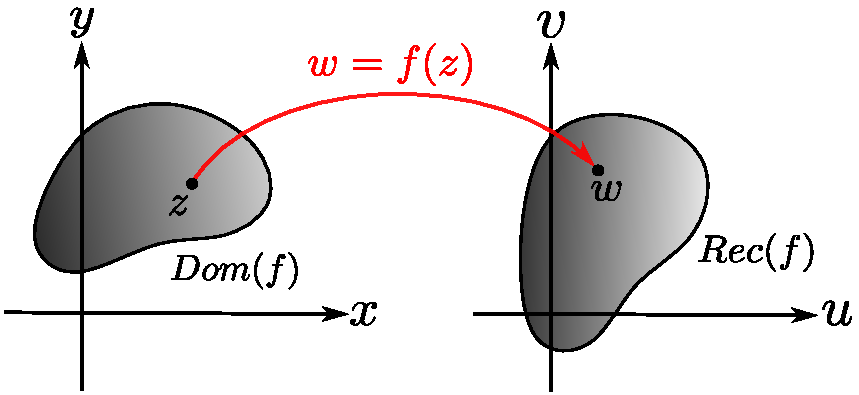
\includegraphics[scale=0.65]{Figuras/FuncionDomRec.pdf}
    \caption{Gráfica del dominio y recorrido de una función compleja.}
    \label{FUncionCompleja}
\end{figure}

\begin{ejemplo}
Consideremos la función $f(z) = iz$ y analicemos la imagen de la circunferencia
$$C_r = \{z \in \mathbb{C} : |z| = r \}; ~ r > 0.$$

Si $z = r (\cos \theta + i \sin \theta) \in C_r$, entonces
\begin{eqnarray*}
f(z) &=& iz \\
&=& \left( \cos \frac{\pi}{2} + i \sin \frac{\pi}{2} \right) r (\cos \theta + i \sin \theta) \\
&=& r \left[ \cos\left( \theta + \frac{\pi}{2} \right) + i \sin \left( \theta + \frac{\pi}{2}  \right) \right] = w.
\end{eqnarray*}

Luego, la imagen $w$ tiene igual magnitud que $z$ y ha sido rotada en $\frac{\pi}{2}$ radianes. En consecuencia,
$$f(C_r) = C_r.$$
\end{ejemplo}

\begin{ejemplo}
Bosqueje la imagen de los conjuntos dados respecto de las funciones:

\begin{enumerate}
\item $f(z) = |z| + i Im(z), ~ C_r$.

\item $f(z) = z^2, ~ B = \{z = (x,y) : 0 \leq x \leq y\}$.
\end{enumerate}

\textbf{Solución:}

\begin{enumerate}
\item La gráfica del dominio y el recorrido están dadas a continuación.

\begin{figure}[H]
    \centering
    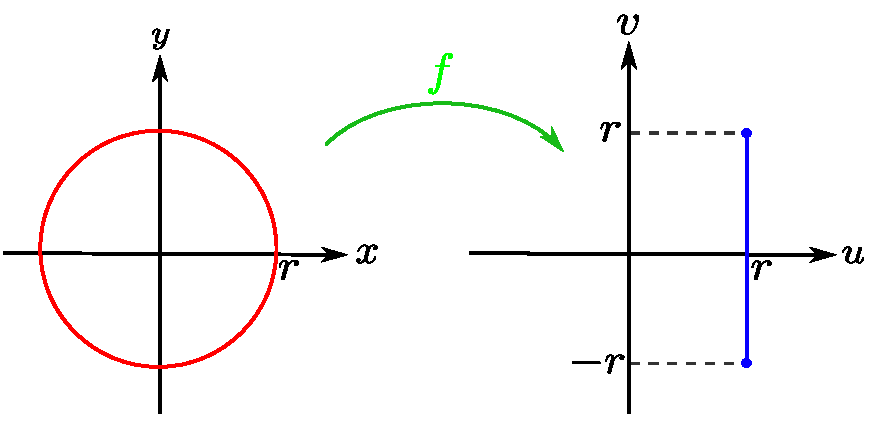
\includegraphics[scale=0.6]{Figuras/EjemploFuncion1.pdf}
    \caption{Imagen de la circunferencia centrada en el origen de radio $r$ para $f(z) = |z| + i Im(z)$.}
    \label{EjemploFuncion1}
\end{figure}

\item Si $z = r e^{i\theta} \in B\setminus \{0\}$, entonces
$$f(z) = z^2 = r^2 e^{i2\theta}$$

con 
$$\frac{\pi}{4} \leq \theta \leq \frac{\pi}{2} \Leftrightarrow \frac{\pi}{2} \leq 2\theta \leq \pi.$$

Como $f(0) = 0$, $f(B) = \{ z= (x,y) : x \leq 0, y \geq 0\}$ y la gráfica del dominio y el recorrido nos queda:

\begin{figure}[H]
    \centering
    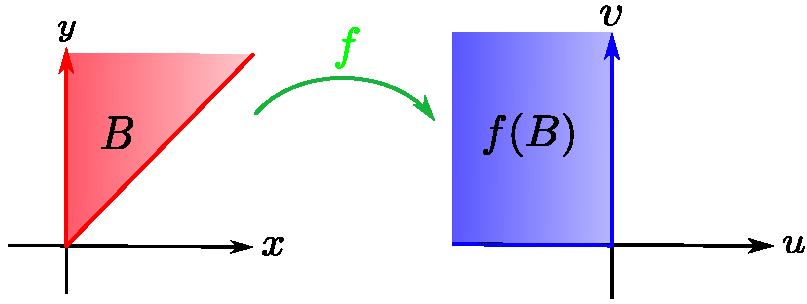
\includegraphics[scale=0.7]{Figuras/EjemploFuncion2.pdf}
    \caption{Imagen de $B$ para $f(z) = z^2$.}
    \label{EjemploFuncion2}
\end{figure}

\end{enumerate}
\end{ejemplo}

\section{Límites} 

\begin{defi}
Sea $f: A \subseteq \mathbb{C} \longrightarrow \mathbb{C}$ una función compleja y sea $z_0 \in \mathbb{C}$ un punto de acumulación de $A$. Diremos que $f$ se aproxima a $w_0$ cuando $z \in A$ se aproxima a $z_0$ si
\begin{equation}
(\forall \varepsilon >0 )(\exists \delta >0) (0 < |z-z_0| < \delta ~\wedge~ z \in A ~\Rightarrow~ |f(z) -w_0| < \varepsilon). \label{defiLimite}
\end{equation}

Denotaremos a \eqref{defiLimite} por
$$\lim_{z \to z_0} f(z) = w_0.$$
\end{defi}

\textbf{Observación:} Notemos que \eqref{defiLimite} puede reescribirse en los siguientes términos:
$$(\forall \varepsilon >0 )(\exists \delta >0) (z \in (B(z_0, \delta)\setminus \{z_0\}) \cap A ~\Rightarrow~ f(z) \in B(w_0, \varepsilon))$$

y geométricamente, se ve como sigue:

\begin{figure}[H]
    \centering
    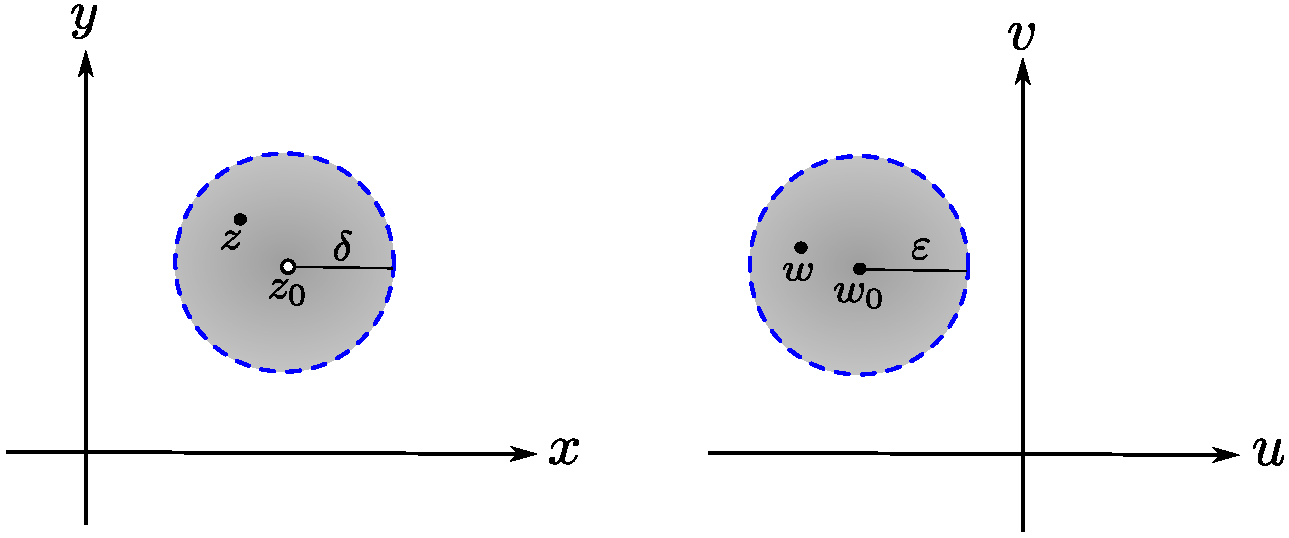
\includegraphics[scale=0.5]{Figuras/DefLimite.pdf}
    \caption{Interpretación geométrica del límite.}
    \label{DefLimite}
\end{figure}

\begin{ejemplo}
Demuestre que
$$\lim_{z \to 1} \frac{iz}{2} = \frac{i}{2}.$$

\textbf{Solución:} En efecto, notemos primero que $A =  \mathbb{C}$, luego para cualquier $\varepsilon > 0$, debemos ser capaces de encontrar $\delta >0$ de manera que si $0 < |z-1| < \delta$, entonces
$$\left| \frac{iz}{2} - \frac{i}{2}\right| < \varepsilon.$$

Trabajando la expresión
$$\left| \frac{iz}{2} - \frac{i}{2}\right| = \left| \frac{i}{2} (z-1) \right| = \frac{1}{2} |z-1|.$$

Luego, eligiendo $\delta = 2\varepsilon$, tenemos para $0 < |z-1|< 2\varepsilon$ que
$$\left| \frac{iz}{2} - \frac{i}{2}\right| =  \frac{1}{2} |z-1| < \frac{1}{2} 2 \varepsilon = \varepsilon.$$
\end{ejemplo}

\textbf{Observación:} Notemos que una función compleja $f: A \subseteq \mathbb{C} \longrightarrow \mathbb{C}$ no es otra cosa que una función $f: A \subseteq \mathbb{R}^2 \longrightarrow \mathbb{R}^2$, asi que todo lo que se estudió en el curso de Cálculo III es aplicable a estas funciones.
\\

En el ejemplo,
$$f(z) = f(x,y) = \frac{1}{2}(0,1)(x,y) = \frac{1}{2}(-y,x)$$

y
$$z \to 1 ~\Rightarrow~ (x,y) \to (1,0).$$

Así,
$$\lim_{z \to 1} f(z) = \lim_{(x,y) \to (1,0)} \frac{1}{2} (-y,x) = \frac{1}{2}(0,1) = \frac{i}{2}.$$

\begin{ejemplo}
Mostrar que
$$\lim_{z \to 2i} (2x+iy^2)= 4i.$$

\textbf{Solución:}
\begin{equation*}
\lim_{z \to 2i} (2x+iy^2) = \lim_{(x,y) \to(0,2)} (2x,y^2) 
= (0,4) = 4i.
\end{equation*}

\end{ejemplo}

\begin{teorema}[Existencia y unicidad del límite]
Si $\lim\limits_{z \to z_0} f(z) = w_0$ y $\lim\limits_{z \to z_0} f(z) = w_1$, entonces $w_0 = w_1$.
\end{teorema}

\begin{proof}
Por hipótesis, dado $\varepsilon >0$, existen $\delta_1>0$ y $\delta_2 >0$ tales que 
\begin{eqnarray*}
0< |z-z_0| < \delta_1 ~\wedge~ z \in Dom(f) ~\Rightarrow ~ |f(z)-w_0| < \frac{\varepsilon}{2}, \\
0< |z-z_0| < \delta_2 ~\wedge~ z \in Dom(f) ~\Rightarrow ~ |f(z)-w_1| < \frac{\varepsilon}{2}.
\end{eqnarray*}

Escogemos $\delta = \min\{\delta_1, \delta_2\}$ (para que ambas condiciones  se verifiquen) y se cumple que
\begin{eqnarray*}
|w_0-w_1| &=& |(f(z) - w_0) - (f(z) - w_1)| \\
&\leq & |f(z) - w_0| + |f(z) - w_1| < \varepsilon .
\end{eqnarray*}

Como $\varepsilon$ es un número positivo arbitrario, tenemos que $|w_1 - w_2|$ es una cota inferior de $]0, + \infty[$. Entonces, por el axioma del supremo, existe $ \inf]0, + \infty[$ y 
$$|w_1 - w_2| \leq  \inf]0, + \infty[ = 0 \Rightarrow  0 \leq |w_1 - w_2| \leq 0 ~\Rightarrow~ |w_1 - w_2| = 0 ~\Rightarrow~ w_1 = w_2.$$

\end{proof}

\begin{propo} \label{LimitesParteRealIm}
Supongamos que $f(z) = u(x,y) +i v(x,y)$, $z_0 = x_0 +iy_0$ y $w_0 = u_0 +iv_0$. Entonces,
$$\lim_{z \to z_0} f(z) = w_0 ~\Leftrightarrow~ \left\{ \begin{array}{c}
\lim\limits_{(x,y) \to (x_0,y_0)} u(x,y) = u_0 \\
\lim\limits_{(x,y) \to (x_0,y_0)} v(x,y) = v_0
\end{array} \right. .$$
\end{propo}

\begin{proof}
En Cálculo III se estudió que las normas 
$$\norm{(x,y)}_2 = \sqrt{x^2+ y^2}~~\mbox{y}~~\norm{(x,y)}_{\infty} = \max\{|x|,|y|\}$$

satisfacen las desigualdades
\begin{eqnarray}
\norm{(x,y)}_{\infty} = \max\{|x|,|y|\} &\leq & \norm{(x,y)}_2. \label{limite1} \\
\norm{(x,y)}_2 &\leq & \sqrt{2} \norm{(x,y)}_{\infty}.\label{limite2}
\end{eqnarray} 

Supongamos que $\lim\limits_{z \to z_0} f(z) = w_0$. Entonces, dado $\varepsilon > 0$, $\exists \delta > 0$ tal que
$$0< |z-z_0| < \delta, z \in Dom(f) ~\Rightarrow ~ |f(z)-w_0| < \varepsilon. $$

Como $|z-z_0| = \norm{(x,y) - (x_0,y_0)}_2$ y 
$$|u(x,y) - u_0| \leq |f(z) - w_0| ~\wedge~|v(x,y) - v_0| \leq |f(z) - w_0|, $$

se verifica que
\begin{eqnarray*}
0< \norm{(x,y) - (x_0,y_0)}_2 < \delta, (x,y) \in Dom(f) ~\Rightarrow ~ |u(x,y) - u_0| \leq |f(z) - w_0| < \varepsilon . \\
0< \norm{(x,y) - (x_0,y_0)}_2 < \delta, (x,y) \in Dom(f) ~\Rightarrow ~ |v(x,y) - v_0| \leq |f(z) - w_0| < \varepsilon . 
\end{eqnarray*}

Hemos probado así, la implicancia hacia la derecha.

Supongamos ahora que
$$\lim_{(x,y) \to (x_0,y_0)} u(x,y) = u_0  ~~\mbox{y}~~\lim_{(x,y) \to (x_0,y_0)} v(x,y) = v_0.$$

Es decir, dado $\varepsilon >0$, $\exists \delta_1, \delta_2 >0$ tales que
\begin{eqnarray*}
0< \norm{(x,y) - (x_0,y_0)}_2 < \delta_1 , (x,y) \in Dom(f) ~\Rightarrow ~ |u(x,y) - u_0| < \frac{\varepsilon}{\sqrt{2}}, \\
0< \norm{(x,y) - (x_0,y_0)}_2 < \delta_2 , (x,y) \in Dom(f) ~\Rightarrow ~ |v(x,y) - v_0|  < \frac{\varepsilon}{\sqrt{2}} . 
\end{eqnarray*}

Escogiendo $\delta = \min\{\delta_1, \delta_2\}$, se verifica:
\begin{eqnarray*}
0 < |z - z_0| = \norm{(x,y) - (x_0,y_0)}_2 < \delta, z \in Dom(f) &\Rightarrow & |f(z) -w_0| \\
&=& \norm{(u(x,y), v(x,y)) - (u_0,v_0)}_2 \\
&\leq & \sqrt{2} \max\{|u(x,y) -u_0|, |v(x,y) - v_0|\} \\
&< & \sqrt{2} \frac{\varepsilon}{\sqrt{2}} = \varepsilon.
\end{eqnarray*}

Hemos probado así, la implicancia hacia la izquierda.

\end{proof}

\begin{teorema}[Álgebra de límites] \label{AlgebraLimites}
Supongamos que
$$\lim_{z \to z_0} f(z) = w_0 ~~\mbox{y}~~ \lim_{z \to z_0} F(z)= W_0.$$

Entonces,

\begin{enumerate}
\item $\lim\limits_{z \to z_0} [f(z) + F(z)] = w_0 + W_0.$

\item $\lim\limits_{z \to z_0} [f(z)  F(z)] = w_0  W_0.$

\item $\lim\limits_{z \to z_0} \left[ \frac{f(z)}{F(z)} \right] = \frac{w_0}{W_0}$, siempre que $W_0 \neq 0$.
\end{enumerate}
\end{teorema}

\begin{proof}
\

\begin{enumerate}

\item Por hipótesis, tenemos que dado $\varepsilon >0$, $\exists \delta_1, \delta_2 >0$ tales que
\begin{eqnarray*}
 0 < |z-z_0| <  \delta_1, z \in Dom(f+F) ~\Rightarrow~ |f(z) - w_0| < \frac{\varepsilon}{2},\\
  0 < |z-z_0| <  \delta_2, z \in Dom(f+F) ~\Rightarrow~ |F(z) - W_0| < \frac{\varepsilon}{2}.
\end{eqnarray*}

Eligiendo $\delta = \min\{ \delta_1, \delta_2 \}$:
\begin{eqnarray*}
  0 < |z-z_0| <  \delta, z \in Dom(f+F)  & \Rightarrow & |(f(z) + F(z)) - (w_0 + W_0)| \\
&= & |(f(z) - w_0) + (F(z) - W_0)| \\
& \leq & |f(z) - w_0| + |F(z) - W_0| \\
&< & \frac{\varepsilon}{2} + \frac{\varepsilon}{2} = \varepsilon.
\end{eqnarray*}

\item Escribamos
\begin{eqnarray*}
|f(z)F(z) - w_0 W_0| &\leq & |f(z)F(z) - f(z)W_0| +|f(z)W_0 - w_0 W_0| \\
&=& |f(z)| |F(z) -W_0| + |f(z) - w_0||W_0|.
\end{eqnarray*}

Queremos estimar cada término. Para hacerlo, la hipótesis nos permite escoger $\delta_1 > 0$ tal que
$$0 < |z-z_0| < \delta_1, z \in Dom(f\cdot F) ~\Rightarrow~ |f(z) -w_0| < 1 ~\Rightarrow~ |f(z)| < |w_0| + 1.$$

Dado $\varepsilon >0$, podemos escoger $\delta_2 > 0$, tal que
$$0 <|z-z_0| < \delta_2, z \in Dom(f\cdot F) ~\Rightarrow~ |f(z)-w_0| < \left\{ \begin{array}{cl}
\frac{\varepsilon}{2 |W_0|},& W_0 \neq 0 \\
1,& W_0 = 0
\end{array} \right. .$$

y $\delta_3 >0$ tal que
$$0 < |z-z_0| < \delta_3,  z \in Dom(f\cdot F)  ~\Rightarrow~ |F(z) -W_0| < \frac{\varepsilon}{2(|w_0| +1)}.$$

Sea $\delta = \min\{\delta_1, \delta_2, \delta_3\}$, entonces
\begin{eqnarray}
0 < |z-z_0| < \delta, z \in Dom(f\cdot F) &\Rightarrow & |f(z)F(z) - w_0 W_0| \nonumber \\
&\leq & |f(z)| |F(z) -W_0| + |f(z) - w_0||W_0| \nonumber \\
&< & \frac{\varepsilon}{2(|w_0| +1)}|f(z)| + \frac{\varepsilon}{2|W_0|} |W_0 | ~~~ (W_0 \neq 0)\label{producto} \\
&< & \frac{\varepsilon}{2} + \frac{\varepsilon}{2} = \varepsilon. \nonumber
\end{eqnarray}

Si en \eqref{producto}, $W_0 = 0$, se reemplaza el segundo término por cero, cumpliéndose también la definición de límite para el producto.

\item Demostremos primero que
$$\lim_{z \to z_0} \left[ \frac{1}{F(z)} \right] = \frac{1}{W_0}, \quad W_0 \neq 0. $$

Por hipótesis, $\exists \delta_1 >0$ tal que
\begin{eqnarray*}
0 < |z-z_0| < \delta_1, z \in Dom(1/F) &\Rightarrow & |F(z) -W_0| < \frac{|W_0|}{2} \\
& \Rightarrow & ||F(z)| - |W_0|| < \frac{|W_0|}{2} \\
& \Leftrightarrow &  - \frac{|W_0|}{2} + |W_0|    < |F(z)| < \frac{|W_0|}{2} + |W_0| \\
& \Rightarrow & \frac{|W_0|}{2} < |F(z)|  ~ \Rightarrow  \frac{1}{|F(z)|} < \frac{2}{|W_0|}.
\end{eqnarray*}

Dado $\varepsilon >0$, $\exists \delta_2 > 0$ tal que
$$0 < |z-z_0| < \delta_2, z \in Dom(1/F) ~ \Rightarrow ~  |F(z)-W_0| < \frac{|W_0|^2}{2} \varepsilon .$$

Escogiendo $\delta = \min \{\delta_1, \delta_2\}$, se verifica que
\begin{eqnarray*}
0 < |z-z_0| < \delta, z \in Dom(1/F) &\Rightarrow & \left| \frac{1}{F(z)} -\frac{1}{W_0}  \right| \\
&=& \frac{1}{|F(z)|} \frac{1}{|W_0|} |F(z) -W_0| \\
&< & \frac{2}{|W_0|^2} \cdot \frac{|W_0|^2}{2} \varepsilon  = \varepsilon . 
\end{eqnarray*}

Luego, por lo demostrado en el ítem $2.$, se tiene que
$$\lim_{z \to z_0} \left[ \frac{f(z)}{F(z)} \right] =\lim_{z \to z_0} \left[ f(z) \cdot \frac{1}{F(z)} \right] = \frac{w_0}{W_0}. $$
\end{enumerate}
\end{proof}

\begin{propo}
$$\lim_{z \to z_0} f(z) = w_0 \Rightarrow\lim_{z \to z_0} |f(z)| = |w_0|. $$
\end{propo}

\begin{proof}
Por hipótesis, dado $\varepsilon >0$, $\exists \delta >0$ tal que
$$0 < |z-z_0| < \delta, z \in Dom(f) ~\Rightarrow ~ |f(z) - w_0| < \varepsilon. $$

Luego,
\begin{eqnarray*}
0 < |z-z_0| < \delta, z \in Dom(f) &\Rightarrow & ||f(z)| - |w_0||  \\
&\leq & |f(z) -w_0| < \varepsilon.
\end{eqnarray*}
\end{proof}

\begin{defi}
Sea $f: A \subseteq \mathbb{C} \longrightarrow \mathbb{C}$ una función compleja y supongamos que $\infty$ es punto de acumulación de $A$. Entenderemos por
$$\lim_{z \to \infty} f(z) = L$$

a lo siguiente:
$$(\forall \varepsilon >0)(\exists M >0)(|z|> M ~\wedge~ z \in A ~\Rightarrow~ |f(z) -L| < \varepsilon).$$
\end{defi}

\begin{ejemplo}
Mostrar que 
$$\lim_{z \to \infty} \frac{1}{z} = 0.$$

\textbf{Solución:} Dado $\varepsilon >0$,  elegimos $M = \frac{1}{\varepsilon} > 0$ tal que
$$|z| > M ~\Rightarrow~ \left| \frac{1}{z} -0 \right| = \left| \frac{1}{z} \right| = \frac{1}{|z|} < \frac{1}{M} = \varepsilon
.$$
\end{ejemplo}


\begin{defi}
Sea $f: A \subseteq \mathbb{C} \longrightarrow \mathbb{C}$ una función compleja y sea $z_0 \in \mathbb{C}$ un punto de acumulación de $A$. Entenderemos por
$$\lim_{z \to z_0} f(z) = \infty$$

a lo siguiente:
$$(\forall M >0)(\exists \delta >0)(0 < |z-z_0| < \delta ~\wedge~ z \in A ~\Rightarrow ~ |f(z)| >M).$$
\end{defi}

\begin{ejemplo}
Mostrar que 
$$\lim_{z \to 0} \frac{1}{z} = \infty.$$

\textbf{Solución:} Dado $M >0$,  elegimos $\delta = \frac{1}{M} > 0$ tal que
$$0 < |z-0| < \delta ~\Rightarrow~ \left| \frac{1}{z} -0 \right| = \left| \frac{1}{z} \right| = \frac{1}{|z|} > M
.$$
\end{ejemplo}

\textbf{Observación:} Existe una definición similar para
$$\lim_{z \to \infty} f(z) = \infty$$

cuando $\infty$ es punto de acumulación de $A$ y que significa:
$$(\forall M >0)(\exists K >0) (|z|> K ~\wedge~ z \in A ~\Rightarrow~ |f(z)| > M).$$

\section{Continuidad}

\begin{defi}
Sea $f: A \subseteq \mathbb{C} \rightarrow \mathbb{C}$ una función compleja y $z_0 \in A$. Diremos que $f$ es \textbf{continua} en $z_0$ si
$$\lim_{z \to z_0} f(z) = f(z_0),$$

o, equivalentemente, 
$$(\forall \varepsilon >0)(\exists \delta >0)(0 < |z-z_0| < \delta ~\wedge~ z \in A ~\Rightarrow~ |f(z) - f(z_0)| < \varepsilon).$$
\end{defi}

\textbf{Observación:} Al igual que antes, al considerar a $f$ como una función $f: A \subseteq \mathbb{R}^2 \longrightarrow \mathbb{R}^2$, usaremos toda información relacionada a la continuidad estudiada en Cálculo III.
\\

Decimos que una función $f: A\subseteq \mathbb{C} \rightarrow \mathbb{C}$ es continua en $A$, o simplemente continua, si $f$ es continua en cada $z_0 \in A$.

\begin{ejemplo}
Demuestre la continuidad de $f(z) = z^2 + b $, con $b \in \mathbb{C}$ constante.
\\

\textbf{Solución:} Hay que demostrar que 
$$\lim_{z \to z_0}( z^2+b) = z_0^2 +b.$$

Primero desarrollemos la expresión
$$|z^2 +b - (z_0^2 + b)| = |z^2 -z_0^2| = |z+z_0| \, |z-z_0|.$$

Acotemos $|z+z_0|$, para ello elegimos $\delta < 1$ tal que $|z-z_0|< 1$ y así
$$|z+z_0| = |z-z_0 + 2z_0| \leq |z-z_0| + 2|z_0| < 1 + 2|z_0|$$

y si además, dado $\varepsilon >0$, elegimos $\delta < \min \left\{1, \frac{\varepsilon}{1+2|z_0|} \right\}$, tenemos que
\begin{eqnarray*}
0 < |z-z_0| < \delta &\Rightarrow & |z^2 +b - (z_0^2 + b)| \\
&=& |z+z_0| \, |z-z_0| \\
&< & (1+2|z_0|) |z-z_0| \\
&<& (1+2|z_0|) \frac{\varepsilon}{1+2|z_0|} = \varepsilon.
\end{eqnarray*}
\end{ejemplo}

\begin{teorema}[Álgebra y composición de funciones continuas]
Sean $f: A \subseteq \mathbb{C} \rightarrow \mathbb{C}$ y $g: A \subseteq \mathbb{C} \rightarrow \mathbb{C} $ dos funciones complejas continuas en $z_0 \in A$. Entonces,

\begin{enumerate}
\item $f+g$ es continua en $z_0$.

\item $f\cdot g$ es continua en $z_0$. 

\item $\frac{f}{g}$ es continua en $z_0$, siempre que $g(z_0) \neq 0$.

\item Si $h: B \subseteq \mathbb{C} \rightarrow \mathbb{C}$ es tal que $h \circ f$ existe y $h$ es continua en $f(z_0)$, entonces $h \circ f$ es continua en $z_0$.
\end{enumerate}
\end{teorema}

\begin{proof}
Los ítems $1.$, $2.$ y $3.$ son consecuencias directas del teorema \ref{AlgebraLimites}.
\\

Para demostrar el ítem $4.$, supongamos que $\lim\limits_{z \to z_0} f(z) = f(z_0)$ y $\lim\limits_{w \to w_0} h(w) = h(w_0)$, con $w_0 = f(z_0)$. 

Entonces, dado $\varepsilon > 0$, $\exists \delta >0$ tal que
\begin{equation*}
 0 < |w-w_0| < \delta, w \in B ~\Rightarrow~ |h(w) - h(w_0)| < \varepsilon.
\end{equation*}

Luego, del $\delta$ escogido, $\exists \delta^* >0$ tal que
\begin{equation*}
 0 < |z-z_0| < \delta^*, z \in A ~\Rightarrow~ |f(z) - f(z_0)| < \delta.
\end{equation*}

Eligiendo $\bar{\delta} = \delta^*$, se verifica:
\begin{eqnarray*}
 0 < |z-z_0| < \bar{\delta}, \, z \in A &\Rightarrow &  |f(z) - f(z_0)| = |w-w_0| < \delta, w \in B  \\
 &\Rightarrow & |h(f(z)) - h(f(z_0))| = |h(w) - h(w_0)| < \varepsilon .
\end{eqnarray*}

Por lo tanto, $\lim\limits_{z \to z_0} (h\circ f)(z) = (h \circ f)(z_0)$.

\end{proof}

\section{Derivadas}

\begin{defi}
Sea $f: A \subseteq \mathbb{C} \rightarrow \mathbb{C}$ y $z_0$ un punto interior de $A$. Definiremos la \textbf{derivada} de $f$ en $z_0$, y escribiremos $f'(z_0)$, a la ecuación
\begin{equation}
f'(z_0) = \lim_{z \to z_0} \frac{f(z) - f(z_0)}{z-z_0},\label{derivada}
\end{equation}

cuando este límite exista. Diremos que $f$ es \textbf{derivable} o \textbf{diferenciable} en $z_0$ cuando la derivada exista.
\end{defi}

\textbf{Observación:} Si denotamos por
$$\Delta z = z-z_0,$$

entonces podemos escribir \eqref{derivada} como
$$f'(z_0) = \lim_{\Delta z \to 0} \frac{f(z_0 + \Delta z) - f(z_0)}{\Delta z}.$$

Nótese que al ser $z_0$ un punto interior,  $f$ está definida en un entorno de $z_0$ y así el número $f(z_0 + \Delta z)$ está siempre definido para $|\Delta z|$ suficientemente pequeño. 

\begin{figure}[H]
    \centering
    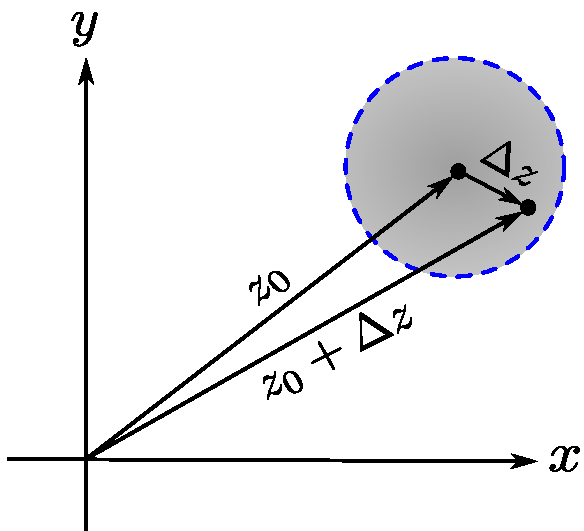
\includegraphics[scale=0.55]{Figuras/DefDerivada.pdf}
    \caption{Interpretación geométrica de la derivada.}
    \label{GeoDerivada}
\end{figure}

Introduciendo el número
$$\Delta w = f(z + \Delta z) - f(z),$$

que denota el cambio en el valor de $f$ correspondiente a un cambio $\Delta z$ en el punto en el que evaluamos $f$. Otra notación para expresar la derivada de $f$ en $z$ es la siguiente:
$$f'(z) = \frac{dw}{dz} = \lim_{\Delta z \to 0} \frac{\Delta w}{\Delta z}.$$

\begin{ejemplo}
Estudiemos la diferenciabilidad de $f(z) = z^2$:
$$\frac{dw}{dz} = \lim_{\Delta z \to 0} \frac{(z + \Delta z)^2 -z^2}{\Delta z} = \lim_{\Delta z \to 0} (2z + \Delta z) = 2z, \quad z \in \mathbb{C}.$$
\end{ejemplo}

\begin{ejemplo}
Estudiemos ahora la diferenciabilidad de $f(z) = |z|^2$:
\begin{eqnarray*}
\frac{\Delta w}{\Delta z} = \frac{f(z + \Delta z) - f(z)}{\Delta z} &=& \frac{|z + \Delta z|^2 - |z|^2}{\Delta z} \\
&=& \frac{(z+\Delta z)\overline{(z+\Delta z)} - z \bar{z}}{\Delta z} \\
&=& \frac{(z+\Delta z)(\bar{z}+\overline{\Delta z}) - z \bar{z}}{\Delta z} \\
&=& \bar{z} + \overline{\Delta z} + z \frac{\overline{\Delta z}}{\Delta z}.
\end{eqnarray*}

Así,
$$f'(0) = \lim_{\Delta z \to 0} \frac{f(0 + \Delta z) - f(0)}{\Delta z} = \lim_{\Delta z \to 0} \overline{\Delta z} =  0.$$

Pero si $z \neq 0$, consideremos las siguientes trayectorias:
$$B_1 = \{z \in \mathbb{C} : Im(\Delta z) = 0\}, \quad B_2 = \{z \in \mathbb{C} : Re(\Delta z) = 0\}$$

tales que $0 \in B_1' \cap B_2'$. Luego,
\begin{eqnarray*}
\lim_{\overset{\Delta z \to 0}{\Delta z \in B_1}} \left[ \bar{z} + \overline{\Delta z} + z \frac{\overline{\Delta z}}{\Delta z} \right] &=& z + \bar{z}, \\
\lim_{\overset{\Delta z \to 0}{\Delta z \in B_2}}\left[ \bar{z} + \overline{\Delta z} + z \frac{\overline{\Delta z}}{\Delta z}\right]&=& -z + \bar{z}. 
\end{eqnarray*}

Por lo tanto, $\frac{dw}{dz}$ no existe para $z \neq 0$.
\end{ejemplo}

\textbf{Observación:} Notemos que al analizar la función $f(z)  = |z|^2$ como función de $\mathbb{R}^2$, tenemos que su parte real e imaginaria, respectivamente, son:
$$u(x,y) = x^2 + y^2, \quad v(x,y) = 0.$$

Ambas tienen derivadas parciales continuas, por tanto, la función \underline{real} es diferenciable en todo punto $(x,y) \in \mathbb{R}^2$.

\begin{ejemplo}
Las derivadas de $f(z) = c = cte$ y $g(z) = z$ son $f'(z) = 0$ y $g'(z) = 1$, respectivamente.
\end{ejemplo}

\begin{propo}
Una función compleja que es diferenciable en un punto $z_0$, ella es continua en este punto.
\end{propo}

\begin{proof}
Sea $f: A \subseteq \mathbb{C} \rightarrow \mathbb{C}$ y $z_0 \in int(A)$. Por hipótesis, 
$$\lim_{z \to z_0}\frac{f(z) -f(z_0)}{z-z_0} = f'(z_0)$$

existe. Luego,
$$\lim_{z \to z_0 } [f(z) - f(z_0)] = \lim_{z \to z_0} \left[ \frac{f(z) -f(z_0)}{z-z_0} (z-z_0) \right] = 0 ~\Rightarrow~ \lim_{z \to z_0 }f(z)  = f(z_0). $$

Por lo tanto, $f$ es continua en $z_0.$

\end{proof}

\textbf{Observación:} El recíproco no es verdadero, ya que $f(z) = |z|^2$ es continua para todo $z \in \mathbb{C}$, pero no es diferenciable si $z \neq 0$.

\begin{teorema}[Álgebra de funciones diferenciables]
Sean $f: A \subseteq \mathbb{C} \rightarrow \mathbb{C}$ y $g: A \subseteq \mathbb{C} \rightarrow \mathbb{C}$ dos funciones complejas y diferenciables en $z_0 \in A$. Entonces,

\begin{enumerate}
\item $f+g$ es diferenciable en $z_0$ y
$$(f+g)'(z_0) = f'(z_0) + g'(z_0).$$

\item $fg$ es diferenciable en $z_0$ y
$$(fg)'(z_0) = f'(z_0) g(z_0) + f(z_0) g'(z_0).$$

\item $\frac{f}{g}$ es diferenciable en $z_0$, siempre que $g(z_0) \neq 0$, y
$$\left( \frac{f}{g} \right)'(z_0) = \frac{f'(z_0) g(z_0) - f(z_0)g'(z_0)}{[g(z_0)]^2}.$$
\end{enumerate}
\end{teorema}

\begin{proof}
Supongamos que $f$ y $g$ son diferenciables en $z_0$, es decir,
$$f'(z_0) =\lim_{z \to z_0}\frac{f(z) -f(z_0)}{z-z_0} ~~\mbox{y}~~ g'(z_0) = \lim_{z \to z_0}\frac{g(z) -g(z_0)}{z-z_0} $$

existen.

\begin{enumerate}
\item Entonces,
\begin{eqnarray*}
(f+g)'(z_0) = \lim_{z \to z_0}\frac{(f+g)(z) -(f+g)(z_0)}{z-z_0} &=&  \lim_{z \to z_0}\frac{(f(z) - f(z_0)) + (g(z) - g(z_0))}{z-z_0} \\
&=& \lim_{z \to z_0}\frac{f(z) - f(z_0)}{z-z_0}  + \lim_{z \to z_0}\frac{g(z) -g(z_0)}{z-z_0} \\
&=& f'(z_0) + g'(z_0).
\end{eqnarray*}

Por lo tanto, $f+g$ es diferenciable en $z_0$.

\item Notemos que 
\begin{eqnarray*}
\frac{(fg)(z) - (fg)(z_0)}{z-z_0} &=& \frac{f(z)g(z) - f(z_0)g(z_0)}{z-z_0} \\
&=& \frac{f(z)g(z) - f(z_0) g(z) + f(z_0)g(z) - f(z_0)g(z_0)}{z-z_0} \\
&=& \frac{f(z) - f(z_0)}{z-z_0} g(z) + \frac{g(z) - g(z_0)}{z-z_0} f(z_0).
\end{eqnarray*}

Como $g$ es diferenciable en $z_0$, entonces también es continua en $z_0$. Con ésto en mente, tenemos que
\begin{eqnarray*}
(fg)'(z_0) &=& \lim_{z \to z_0}\frac{(fg)(z) - (fg)(z_0)}{z-z_0} \\
&=& \left( \lim_{z \to z_0}\frac{f(z) -f(z_0)}{z-z_0} \right)\cdot \left( \lim_{z \to z_0} g(z) \right) + f(z_0) \lim_{z \to z_0}\frac{g(z) - g(z_0)}{z-z_0} \\
&=& f'(z_0) g(z_0) + f(z_0) g'(z_0).
\end{eqnarray*}

Por lo tanto, $fg$ es diferenciable en $z_0$.

\item Probemos primero que
$$\left( \frac{1}{g} \right)'(z_0) = - \frac{g'(z_0)}{[g(z_0)]^2}, \quad g(z_0) \neq 0.$$

Para ello, teniendo en cuenta las hipótesis y que $g$ es continua, se tiene que
\begin{eqnarray*}
\left( \frac{1}{g} \right)'(z_0) &=& \lim_{z \to z_0} \frac{\left( \frac{1}{g} \right)(z) - \left(  \frac{1}{g}\right)(z_0)}{z-z_0} \\
&=& \lim_{z \to z_0} \frac{\frac{1}{g(z)} -   \frac{1}{g(z_0)}}{z-z_0} \\
&=& \lim_{z \to z_0} \left[ - \frac{g(z) - g(z_0)}{z-z_0} \cdot \frac{1}{g(z)g(z_0)} \right] \\
&=&  - \frac{g'(z_0)}{[g(z_0)]^2}.
\end{eqnarray*}

Por la regla del producto demostrada en el ítem $2.$, obtenemos que
\begin{eqnarray*}
\left( \frac{f}{g} \right)'(z_0) = \left( f \cdot \frac{1}{g} \right)'(z_0) &=& f'(z_0) \left( \frac{1}{g} \right) (z_0) + f(z_0) \left( \frac{1}{g} \right)'(z_0) \\
&=& \frac{f'(z_0)}{g(z_0)} - \frac{f(z_0)g'(z_0)}{[g(z_0)]^2} \\
&=& \frac{f'(z_0) g(z_0) -f(z_0)g'(z_0) }{[g(z_0)]^2}.
\end{eqnarray*}

Por lo tanto, $\frac{f}{g}$ es diferenciable en $z_0$.
\end{enumerate}
\end{proof}

\begin{teorema}[Regla de la cadena]
Sea $f: A \subseteq \mathbb{C} \rightarrow \mathbb{C}$  diferenciables en $z_0 \in A$. Si $g: B \subseteq \mathbb{C} \rightarrow \mathbb{C}$ es tal que $g \circ f$ existe y $g$ es diferenciable en $f(z_0)$, entonces $g \circ f$ es diferenciable en $z_0$ y 
$$(g \circ f)'(z_0) = g'(f(z_0)) f'(z_0).$$
\end{teorema}

\begin{proof}
Sea $w_0 = f(z_0)$ y defínase, para $w \in B$,
$$h(w) = \left\{ \begin{array}{cl}
\frac{g(w)-g(w_0)}{w-w_0} - g'(w_0),& w \neq w_0 \\
0 ,& w = w_0
\end{array} \right. .$$

Dado que $g'(w_0)$ existe, $h$ es continua. Como la composición de funciones continuas es continua:
$$\lim_{z \to z_0} h(f(z)) = h(w_0) =  0.$$

De la definición de $h$ y haciendo $w = f(z)$, obtenemos que 
$$(g \circ f)(z) - (g\circ f)(z_0) = g(f(z)) - g(w_0) = [h(f(z)) +g'(w_0)][f(z)-w_0].$$

Nótese que esto se satisface aún si $f(z) = w_0$.

Luego, 
\begin{eqnarray*}
(g \circ f)' (z_0) = \lim_{z \to z_0} \frac{(g \circ f)(z) - (g\circ f)(z_0)}{z-z_0}  &=& \lim_{z \to z_0} \left\{ [h(f(z)) +g'(w_0)] \frac{f(z) - f(z_0)}{z-z_0}  \right\}\\
&=& \left( \lim_{z \to z_0}[ h(f(z)) +g'(w_0)] \right) \left( \lim_{z\to z_0} \frac{f(z) - f(z_0)}{z-z_0} \right) \\
&=& g'(f(z_0)) f'(z_0) . 
\end{eqnarray*}

Por lo tanto, $g\circ f$ es diferenciable en $z_0$.

\end{proof}

\begin{ejemplo}
Muestre que
\begin{equation}
\frac{d}{dz}[z^n] = n z^{n-1}, \quad n \in \mathbb{Z}. \label{derivadaZ}
\end{equation}

\textbf{Solución:} Procedemos por inducción.

Para $n = 1$, se tiene que
$$\frac{d}{dz}[z] = 1 = 1 z^{1-1}.$$

Supongamos que para $n \in \mathbb{N}$, se verifica \eqref{derivadaZ}. Probemos que para $n+1$ también se cumple.
\begin{equation*}
\frac{d}{dz}[z^{n+1}] =  \frac{d}{dz}[ z^{n} z] = z \frac{d}{dz}[z^n] + z^n   \frac{d}{dz} [z] = (n+1) z^n.
\end{equation*}

Para $n = 0$, es trivial que se verifica \eqref{derivadaZ}.

Ahora, haciendo $m = -n, n \in \mathbb{N}$, tenemos
\begin{eqnarray*}
\frac{d}{dz}[z^m] = \frac{d}{dz}[z^{-n}] &=& \frac{d}{dz} (z^{-1})^n \\
& =& n (z^{-1})^{n-1} \frac{d}{dz} \left[ \frac{1}{z} \right] \qquad \mbox{(Regla de la cadena)} \\
&=& -n (z^{-1})^{n-1} (z^{-1})^2 \qquad \mbox{(Regla del cociente)} \\
&=& -n (z^{-1})^{n+1} = m z^{m-1}.  
\end{eqnarray*}

De esta manera, hemos probado \eqref{derivadaZ} para todo $n \in \mathbb{Z} $.
\end{ejemplo}

\section{Ecuaciones de Cauchy-Riemann}

Supongamos que
$$f(z) = u(x,y) + iv(x,y)$$

es derivable en $z_0 = x_0 + iy_0$, es decir,
\begin{eqnarray*}
f'(z_0) &=& \lim_{\Delta z \to 0} \frac{f(z_0 + \Delta z) - f(z_0)}{\Delta z} \\
&=& \lim_{\Delta z \to 0} \frac{u(x_0 + \Delta x, y_0 + \Delta y) - u(x_0,y_0) + i [v(x_0 + \Delta x, y_0 + \Delta y) - v(x_0,y_0)]}{\Delta x + i \Delta y} 
\end{eqnarray*}

existe, con $\Delta z = \Delta x + i \Delta y$.

En particular, si escogemos una trayectoria de tal forma que $Im(\Delta z) = \Delta y = 0$, tenemos que $\Delta z= \Delta x + i0 = \Delta x$ y 
\begin{eqnarray*}
\lim_{\Delta x \to 0} \frac{u(x_0 + \Delta x, y_0) -u(x_0,y_0)}{\Delta x} &=& u_x(x_0,y_0) ; \\
\lim_{\Delta x \to 0} \frac{i[v(x_0 + \Delta x, y_0) -v(x_0,y_0)]}{\Delta x} &=& i v_x(x_0,y_0) .
\end{eqnarray*}

Así,
\begin{equation}
f'(z_0) = u_x(x_0,y_0) + i v_x(x_0,y_0). \label{CR1}
\end{equation}

Por otro lado, si escogemos una trayectoria de tal forma que $Re(\Delta z) = \Delta x = 0$, tenemos que $\Delta z = 0 + i \Delta y = i \Delta y$ y 
\begin{eqnarray*}
\lim_{\Delta y \to 0} \frac{u(x_0, y_0 + \Delta y) -u(x_0,y_0)}{i \Delta y} &=& - iu_y(x_0,y_0) ;  \\
\lim_{\Delta y \to 0} \frac{i[v(x_0, y_0 + \Delta y) -v(x_0,y_0)]}{i \Delta y} &=&  v_y(x_0,y_0) .
\end{eqnarray*}

Así,
\begin{equation}
f'(z_0) = v_y(x_0,y_0) - i u_y(x_0,y_0). \label{CR2}
\end{equation}

De \eqref{CR1} y \eqref{CR2} podemos concluir que
\begin{equation}
\left\{ \begin{array}{ccc}
u_x(x_0,y_0)& =& v_y(x_0,y_0) \\
u_y(x_0,y_0) &=& - v_x(x_0,y_0)
\end{array} \right. . \label{CR3}
\end{equation}

Las ecuaciones de \eqref{CR3} se llaman \textbf{ecuaciones de Cauchy-Riemann} y se resumen en el siguiente teorema.

\begin{teorema}
Supongamos que 
$$f(z) = u(x,y) + i v(x,y)$$

y que $f'(z_0)$ existe en el punto $z_0 = x_0 + iy_0$. Entonces, las derivadas parciales de primer orden de $u$ y $v$ existen en el punto $(x_0,y_0)$ y satisfacen en él las ecuaciones de Cauchy-Riemann
$$ u_x = v_y, \quad u_y = -v_x. $$

Además, $f'(z_0)$ se puede expresar como
$$f'(z_0) = u_x(x_0,y_0) + i v_x(x_0,y_0).$$
\end{teorema}

\begin{ejemplo}
Ilustremos el teorema con la función diferenciable 
$$f(z) = z^2 = (x+iy)^2 =  x^2 - y^2 + i2xy. $$

 En este caso, 
$$u(x,y) = x^2-y^2, ~~ v(x,y) = 2xy.$$

Luego,
\begin{eqnarray*}
u_x(x,y) &=& 2x = v_y(x,y) . \\
u_y(x,y) &=& -2y = -v_x(x,y) .
\end{eqnarray*}
\end{ejemplo}

\begin{ejemplo}
Muestre que la función $f(z) = |z|^2$ no es diferenciable en todo punto, excepto en $z = 0$.
\\

\textbf{Solución:} En este caso,
$$u(x,y) = x^2+y^2, ~~ v(x,y) = 0.$$

Luego,
\begin{eqnarray*}
u_x(x,y) &=& 2x, ~  v_y(x,y) = 0, \\
u_y(x,y) &=& 2y, ~ -v_x(x,y) = 0.
\end{eqnarray*}

Puesto que las ecuaciones de Cauchy-Riemann no se satisfacen salvo si $x = y = 0$, $f$ no es diferenciable en $\mathbb{C} - \{0\}$.
\end{ejemplo}

\textbf{Observación:} EL recíproco del teorema, en general, no es verdadero. Como contraejemplo, consideremos la función
$$f(z) = \left\{ \begin{array}{cll}
\frac{(\bar{z})^2}{z} &,& z \neq 0 \\
0 &,& z = 0
\end{array} \right. .$$

Notemos que para $z = x+iy \neq 0$,
$$\frac{(\bar{z})^2}{z} = \frac{(x-iy)^2}{x+iy} = \frac{(x^2-y^2 -i2xy)(x-iy)}{x^2+y^2} = \color{red} \underbrace{ \color{black} \frac{x^3 - 3xy^2}{x^2+y^2}}_{ \color{red}  u(x,y)} \color{black} + i \color{red} \underbrace{\color{black}\frac{y^3-3x^2y}{x^2+y^2}}_{\color{red} v(x,y)}\color{black}.$$

Luego,
\begin{eqnarray*}
u_x(0,0) &=& \lim_{h \to 0} \frac{u(h,0) - u(0,0)}{h} 
= \lim_{h \to 0} \frac{\frac{h^3}{h^2} - 0}{h} 
 = 1, \\
u_y(0,0) &=& \lim_{h \to 0} \frac{u(0,h) - u(0,0)}{h} 
= \lim_{h \to 0} \frac{0}{h} = 0, \\
v_x(0,0) &=& \lim_{h \to 0} \frac{v(h,0) - v(0,0)}{h} 
= \lim_{h \to 0} \frac{0}{h} = 0, \\
v_y(0,0) &=& \lim_{h \to 0} \frac{v(0,h) - v(0,0)}{h} 
= \lim_{h \to 0} \frac{\frac{h^3}{h^2} - 0}{h} = 1.
\end{eqnarray*}

Podemos observar que $f$ satisface las ecuaciones de cauchy-Riemann en $z= 0$. 

Por otro lado,
$$f'(0) = \lim_{z \to 0} \frac{f(z) - f(0)}{z} =\lim_{z \to 0} \frac{\frac{(\bar{z})^2}{z}}{z} = \lim_{z \to 0} \left( \frac{\bar{z}}{z}  \right)^2. $$

Sean los conjuntos
$$B_1 = \{z \in \mathbb{C} : Re(z) = 0\}, \quad B_2 = \{z \in \mathbb{C} : Re( z) = Im(z)\}$$

tales que $0 \in B_1' \cap B_2'$, tenemos
\begin{eqnarray*}
\lim_{\overset{z \to 0}{z \in B_1}} \left( \frac{\bar{z}}{z}  \right)^2 &=& \lim_{y \to 0} \left( \frac{-iy}{iy} \right)^2 = 1, \\
\lim_{\overset{z \to 0}{z \in B_2}} \left( \frac{\bar{z}}{z}  \right)^2 &=& \lim_{(x,y) \to (0,0)} \left( \frac{x-ix}{x+ix} \right)^2 = \lim_{(x,y) \to (0,0)} \left( \frac{1-i}{1+i} \right)^2 =  \left( \frac{1-i}{1+i} \right)^2.
\end{eqnarray*}

Dado que ambos límites son distintos, $f'(0)$ no existe.
\\

Aún así, tenemos un recíproco, asumiendo ciertas hipótesis.

\begin{teorema} \label{ECR}
Sea $f: A \subseteq \mathbb{C} \rightarrow \mathbb{C}, f(z) = u(x,y) + iv(x,y)$ una función dada, con $A$ un conjunto abierto. Si $u$ y $v$ son diferenciables, en el sentido de las variables reales, y en $(x_0,y_0) = z_0 \in A$ satisfacen las ecuaciones de Cauchy-Riemann, entonces $f'(z_0)$ existe.
\end{teorema}

\begin{proof}
Supongamos que $u$ y $v$ son diferenciables en $A$ y satisfacen las ecuaciones de Cauchy-Riemann en $(x_0,y_0) = z_0$. Entonces, por definición de diferenciabilidad, podemos escribir
\begin{align*}
    u(x,y) - u(x_0,y_0) &= u_x(x_0,y_0) (x-x_0) + u_y(x_0,y_0) (y-y_0) + \varepsilon_1(x,y) \norm{(x-x_0,y-y_0)}, \\
    v(x,y) - v(x_0,y_0) &= v_x(x_0,y_0) (x-x_0) + v_y(x_0,y_0) (y-y_0) + \varepsilon_2(x,y) \norm{(x-x_0,y-y_0)},
\end{align*}

donde $\varepsilon_1(x,y), \varepsilon_2(x,y)$ son funciones que tienden a cero cuando $(x,y) \to (x_0,y_0)$. Sumando ambas expresiones (después de multiplicar la segunda ecuación por $i$), obtenemos
\begin{align*}
    f(x+iy) - f(x_0 + iy_0) &= [u_x(x_0,y_0) + i v_x(x_0,y_0)] (x-x_0) +  [u_y(x_0,y_0) + i v_y(x_0,y_0)] (y-y_0) \\
    &\quad + \varepsilon_1(x,y)  \norm{(x-x_0,y-y_0)} + i \varepsilon_2(x,y)  \norm{(x-x_0,y-y_0)} \\
    &= [u_x(x_0,y_0) + i v_x(x_0,y_0)] (x-x_0) +  [-v_x(x_0,y_0) + i u_x(x_0,y_0)] (y-y_0) \\
    &\quad + \varepsilon_1(x,y)  \norm{(x-x_0,y-y_0)} + i \varepsilon_2(x,y)  \norm{(x-x_0,y-y_0)} \\
    &=  [u_x(x_0,y_0) + i v_x(x_0,y_0)] [(x-x_0) + i (y-y_0)] + E(x+iy) [(x-x_0) + i(y-y_0)],
\end{align*}

donde en la segunda igualdad hemos reemplazado las ecuaciones ecuaciones de Cauchy-Riemann y hemos definido
$$E(x+iy) = \varepsilon_1(x,y) \frac{\norm{(x-x_0,y-y_0)}}{(x-x_0) + i(y-y_0)} + i \varepsilon_2(x,y)  \frac{\norm{(x-x_0,y-y_0)}}{(x-x_0) + i(y-y_0)}.$$

Notemos que 
\begin{align*}
    |E(x+iy)| &\leq \left| \varepsilon_1(x,y) \frac{\norm{(x-x_0,y-y_0)}}{(x-x_0) + i(y-y_0)} \right| +  \left| \varepsilon_2(x,y) \frac{\norm{(x-x_0,y-y_0)}}{(x-x_0) + i(y-y_0)} \right| \\
    &= | \varepsilon_1(x,y)| \cancelto{1}{\frac{\norm{(x-x_0,y-y_0)}}{|(x-x_0) + i(y-y_0)|}} +   | \varepsilon_2(x,y)| \cancelto{1}{\frac{\norm{(x-x_0,y-y_0)}}{|(x-x_0) + i(y-y_0)|}} \\
    &= |\varepsilon_1(x,y)| + |\varepsilon_2(x,y)|.
\end{align*}

Como $\lim\limits_{(x,y) \to (x_0,y_0)} \varepsilon_1(x,y) = \lim\limits_{(x,y) \to (x_0,y_0)} \varepsilon_2(x,y) = 0$, por el teorema del acotamiento,
$$\lim_{(x,y) \to (x_0,y_0)} E(x+iy) = 0.$$

Por lo tanto, 
\begin{align*}
    \lim_{z \to z_0} \frac{f(z)-f(z_0)}{z-z_0} &= \lim_{z \to z_0} \frac{f(x+iy)-f(x_0 + iy_0)}{(x-x_0) + i (y- y_0)} \\ 
    &= \lim_{z \to z_0} \left[ u_x(x_0,y_0) + i v_x(x_0,y_0) \right] + \lim_{z \to z_0} \left[E(x+iy) [(x-x_0) + i(y-y_0)] \right] \\
    &= u_x(x_0,y_0) + i v_x(x_0,y_0),
\end{align*}

ésto es, $f'(z_0)$ existe.

\end{proof}

\textbf{Observación:} Es directo del teorema que si $u_x$, $u_y$, $v_x$ y $v_y$ existen, son continuas en $A$ y satisfacen las ecuaciones de Cauchy-Riemann, entonces $f$ es derivable en $A$.

\begin{ejemplo}
Sea 
$$f(z) = e^x e^{iy} = \color{red}\underbrace{\color{black}e^x \cos y}_{\color{red} u(x,y)} \color{black}+ i \color{red}\underbrace{\color{black}e^x \sin y}_{\color{red}v(x,y)}\color{black}.$$

Sus derivadas parciales son:
\begin{eqnarray*}
u_x(x,y) = e^x \cos y; \quad v_x(x,y) = e^x \sin y \\
u_y(x,y) = - e^x \sin y; \quad v_y(x,y) = e^x \cos y  .
\end{eqnarray*}

Claramente son continuas en cada punto del plano complejo y satisfacen las ecuaciones de Cauchy-Riemann.  Por lo tanto, $f$ es derivable en cada punto del plano y su derivada es 
$$f'(z) = e^x \cos y + i e^x \sin y = e^x e^{iy} = f(z).$$
\end{ejemplo}

\begin{ejemplo}
La función
$$g(z) = |z|^2 = x^2+y^2$$

es derivable en $z_0 = 0$. En efecto,
$$u(x,y) = x^2+y^2, \quad v(x,y) = 0.$$

Así, 
\begin{eqnarray*}
u_x(x,y) = 2x; \quad v_x(x,y) = 0 \\
u_y(x,y) = 2y; \quad v_y(x,y) = 0  
\end{eqnarray*}

son continuas en todo el plano y satisfacen las ecuaciones de Cauchy-Riemann sólo en $(0,0)$.
De esta forma, $f'(0) = 0$.
\end{ejemplo}

\subsection{Coordenadas polares}

Sea 
$$f(z) = u(x,y) + iv(x,y)$$

una función compleja que es derivable en un punto $z$. Luego, en su forma polar, tenemos
\begin{eqnarray*}
f(r \cos\theta, r \sin \theta) &=& u(r \cos\theta, r \sin \theta) + i v(r \cos\theta, r \sin \theta) \\
&=& s(r,\theta) + it(r,\theta)
\end{eqnarray*}

donde 
$$s(r, \theta) = u(x(r,\theta), y(r,\theta)); \quad t(r, \theta) = v(x(r,\theta), y(r,\theta)).$$

Analicemos las ecuaciones de Cauchy-Riemann en su forma polar. Para ello, por regla de la cadena, tenemos que
\begin{eqnarray}
s_r &=& u_x \frac{\partial x}{\partial r } + u_y \frac{\partial y}{\partial r} = u_x \cos \theta + u_y \sin \theta.  \label{Polar1}\\
s_{\theta} &=& u_x \frac{\partial x}{\partial \theta } + u_y \frac{\partial y}{\partial \theta} =  u_x (-r \sin \theta) + u_y (r \cos \theta). \label{Polar2}
\end{eqnarray}

Por otro lado,
\begin{eqnarray}
t_{\theta} &=& v_x \frac{\partial x}{\partial \theta} + v_y \frac{\partial y}{\partial \theta} \\
&=& \color{red}\underbrace{\color{black}v_x}_{\color{red}-u_y} \color{black}(-r \sin \theta) + \color{red}\underbrace{\color{black}v_y}_{\color{red}u_x} \color{black}(r \cos \theta) \label{Polar3}\\
&=& -u_y (-r \sin \theta) + u_x (r \cos \theta)  \\
&=& r [u_x \cos \theta + u_y \sin \theta] = rs_r. 
\end{eqnarray}

y
\begin{eqnarray}
t_{r} &=& v_x \frac{\partial x}{\partial r} + v_y \frac{\partial y}{\partial r} \\
&=& \color{red}\underbrace{\color{black}v_x}_{\color{red}-u_y}\color{black} \cos \theta + \color{red}\underbrace{\color{black}v_y}_{\color{red}u_x} \color{black}\sin\theta \label{Polar4}  \\
&=& -u_y \cos\theta + u_x\sin\theta \\
&=& - \frac{1}{r} s_{\theta}. 
\end{eqnarray}

De esta manera, tenemos que 
\begin{equation}
\boxed{\begin{array}{ccc}
s_r & =& \frac{1}{r}t_{\theta}, \\
s_{\theta} &=& - r t_r.
\end{array}  } \label{ECRPolares}
\end{equation}

Hasta ahora, hemos probado que si $f(z)$ satisface las ecuaciones de cauchy-Riemann, en coordenadas cartesianas, en el punto $z$, entonces son válidas las ecuaciones  \eqref{ECRPolares} en ese mismo punto. De aquí nos podemos preguntar si el recíproco es válido. Para ello, de las ecuaciones \eqref{Polar1} y \eqref{Polar2}, resolvamos el siguiente sistema con incógnitas $u_x$ y $u_y$:
\begin{equation}
\left\{ \begin{array}{ccc}
s_r & =& u_x \cos \theta + u_y \sin \theta \\
s_{\theta} &=&  u_x (-r \sin \theta) + u_y (r \cos \theta)
\end{array} \right.  \Rightarrow \left\{ \begin{array}{ccc}
u_x &=& s_r \cos \theta - s_{\theta} \frac{\sin\theta}{r}\\
u_y &=&  s_{\theta} \frac{\cos \theta}{r} + s_r \sin \theta
\end{array} \right. .
\end{equation}
 
A partir de las ecuaciones \eqref{Polar3} y \eqref{Polar4}, resolvamos este otro sistema pero ahora para las incógnitas $v_x$ y $v_y$:
\begin{equation}
\left\{ \begin{array}{ccc}
t_r & =&  v_x \cos \theta + v_y \sin\theta  \\
t_{\theta} &=& v_x (-r \sin \theta) + v_y (r \cos \theta)
\end{array} \right.  \Rightarrow \left\{ \begin{array}{ccc}
v_x &=& t_r \cos \theta - t_{\theta} \frac{\sin\theta}{r}\\
v_y &=&  t_{\theta} \frac{\cos \theta}{r} + t_r \sin \theta
\end{array} \right.  .
\end{equation}

Suponiendo que $f$ satisface las ecuaciones \eqref{ECRPolares}, tenemos que 
\begin{equation}
\left\{ \begin{array}{ccc}
u_x & =&  s_r \cos \theta - s_{\theta} \frac{\sin\theta}{r} = t_{\theta} \frac{\cos \theta}{r} + t_r \sin \theta = v_y \\
u_y &=&  s_{\theta} \frac{\cos \theta}{r} + s_r \sin \theta = -t_r \cos \theta + t_{\theta} \frac{\sin\theta}{r} = - v_x
\end{array} \right. .
\end{equation}

De esta manera, hemos verificado  que las ecuaciones \eqref{ECRPolares} son las \textit{ ecuaciones de Cauchy-Riemann en forma polar}. Por lo tanto, si $f(r,\theta) = s(r,\theta) + i t(r,\theta)$ satisface las ecuaciones \eqref{ECRPolares} en $(r_0,\theta_0)$ y sus funciones componentes son diferenciables en el sentido real, entonces $f$ es derivable en $(r_0,\theta_0)$.

A partir de lo anterior, podemos escribir
$$f'(z) = e^{-i\theta} [s_r(r,\theta) + it_r (r,\theta)] = \frac{1}{r}e^{-i\theta} [t_{\theta}(r,\theta) - i s_{\theta} (r,\theta)].$$

\begin{ejemplo}
Consideremos la función 
$$f(z) = \frac{1}{z} = \frac{1}{re^{i\theta}}.$$

En este caso,
$$s(r,\theta) = \frac{\cos \theta}{r} ~~\mbox{y}~~ t(r,\theta) = -\frac{\sin \theta}{r}.$$

Sus derivadas parciales son:
\begin{eqnarray*}
s_r = - \frac{\cos \theta }{r^2}; \quad t_r = \frac{\sin\theta}{r^2}; \\
s_{\theta} = - \frac{\sin \theta}{r}; \quad t_{\theta} =  -\frac{\cos\theta}{r}  .
\end{eqnarray*}

Claramente son continuas en cada punto del plano complejo, excepto en el origen. Además, satisfacen la ecuaciones de Cauchy-Riemann. 

Por lo tanto, $f$ es derivable en $\mathbb{C}-\{0\}$ y su derivada está dada por 
$$f'(z) = e^{-i\theta} \left[ - \frac{\cos \theta}{r^2} + i \frac{\sin\theta}{r^2} \right] = - \frac{1}{(re^{i\theta})^2} = -\frac{1}{z^2}.$$

\end{ejemplo}

\section{Funciones analíticas}
 
\begin{defi}
Sea $$f(z) = u(x,y) + iv(x,y)$$ una función compleja. Diremos que

\begin{enumerate}
\item $f$ es una \textbf{función analítica en $z_0$} si $f$ es derivable en una vecindad de $z_0$. En ocasiones, se utiliza el nombre de \textbf{holomórfica} para el mismo concepto.

\item $f$ es \textbf{analítica en su dominio de definición} si $f$ es analítica en cada uno de los puntos del dominio.

\item $f$ es \textbf{entera} si es analítica en todo el plano complejo.
\end{enumerate}
\end{defi}

\begin{ejemplo}
La función $f(z) = |z|^2$ no es analítica en $z_0 = 0$, aunque ésta sea derivable en ese punto. Por otro lado la función $g(z) = z^2$, y en general toda función polinómica, es una función entera.
\end{ejemplo} 

\begin{defi}
Sea $$f(z) = u(x,y) + i v(x,y)$$ una función compleja y $z_0 \in \mathbb{C}$. Diremos que un punto $z_0$ es un \textbf{punto singular de (o singularidad de)} $f$ si no es analítica en $z_0$ o $z_0 \notin Dom(f)$, pero es analítica en algún punto de cualquier vecindad de $z_0$.
\end{defi}

\begin{ejemplo}
La función $f(z) = 1/z$ tiene una singularidad en $z_0 = 0$. En cambio, la función $g(z) = |z|^2$ no tiene singularidades, pues no es analítica en punto alguno.
\end{ejemplo}

\textbf{Observación:} Las derivadas de la suma y del producto de dos funciones existen siempre que ambas funciones tengan derivada. Así pues, \textit{si dos funciones son analíticas en un dominio $D$, su suma y su producto son analíticos ambos en $D$}. Análogamente, \textit{su cociente es analítico en $D$ siempre cuando la función del denominador no se anule en ningún punto de $D$}. Por otro lado, con la regla de la cadena encontramos que \textit{una función compuesta de dos funciones analíticas es analítica}.
\\

Ilustremos con un ejemplo la composición de funciones analíticas.

\begin{ejemplo}
Si 
$$f(z) = z^2 = r^2 e^{i2\theta} ~~\mbox{y}~~ g(z) = \sqrt{r} e^{i \theta /2}; \quad r > 0, - \pi < \theta < \pi$$

ambas analíticas en su dominio. Notemos que el dominio  de $g$ es todo el plano, excepto
$$\{z \in \mathbb{C} : Re(z) \leq 0 ~\wedge~ Im(z) = 0\},$$

es decir, el semi-eje real negativo, incluyendo al origen. Al componer $g \circ f$, su dominio es
$$D = \left\{z \in \mathbb{C} : Re(z) > 0~\wedge~ - \frac{\pi}{2} < \theta < \frac{\pi}{2} \right\},$$

es decir, todo el semiplano a la derecha del eje imaginario, excluyendo a dicho eje. Así
$$g(f(z)) = z $$

es analítica en $D$.
\end{ejemplo}

En el Cálculo integral real aprendimos que si $f'(x) = 0$, entonces $f$ es constante, pero ¿será cierto para el caso complejo?, para responder esta pregunta enunciemos primero un teorema del Cálculo III:

\begin{teorema}[del valor medio en dos dimensiones]
Sea $u$ una función diferenciable en un abierto $A \subseteq \mathbb{R}^2$. Suponga que el segmento $[z_1,z_2]$ que une $z_1 = (x_1,y_1)$ a $z_2 = (x_2,y_2)$ está contenido en $A$. Entonces, existe un punto $z = (x_0,y_0) \in [z_1,z_2]$ tal que
$$u(x_2,y_2) - u(x_1,y_1) = u_x(z) (x_2-x_1) + u_y(z) (y_2-y_1).$$
\end{teorema}

\begin{proof}
Una parametrización del segmento $[z_1,z_2]$ sería
$$x(t) = x_1 + t(x_2-x_1), \quad y(t) = y_1 + t(y_2-y_1), \quad 0 \leq t \leq 1.$$

De aquí, tenemos $x'(t) = x_2-x_1$ e $y'(t) = y_2-y_1$. Definamos la función $U(t) = u(x(t),y(t))$ para $0 \leq t \leq 1$ tal que $U(0) = u(x_1,y_1)$, $U(1) = u(x_2,y_2)$ y, por regla de la cadena,
$$\frac{d U}{dt} = \frac{\partial u}{\partial x}\frac{dx}{dt} + \frac{\partial u}{\partial y}\frac{dy}{dt} = \frac{\partial u}{\partial x}(x_2-x_1)+ \frac{\partial u}{\partial y}(y_2-y_1).$$

Usando el teorema del valor medio en una variable a $U(t)$, existe $t \in ]0,1[$ tal que
$$U(1) - U(0) = \frac{dU}{dt}(t_0) (1-0).$$

Así,
$$u(x_2,y_2) - u(x_1,y_1) = \frac{\partial u}{\partial x}(x(t_0),y(t_0)) (x_2-x_1) + \frac{\partial u}{\partial y}(x(t_0),y(t_0)) (y_2-y_1)$$

y haciendo $z = (x(t_0),y(t_0)) \in [z_1,z_2]$, hemos demostrado el teorema.

\end{proof}

\begin{teorema}
Si $f'(z) = 0$ en todos los puntos de un dominio $D$ (abierto conexo), entonces $f(z)$ es constante sobre $D$.
\end{teorema}

\begin{proof}
Sea $f(z) = u(x,y) + i v(x,y)$. Entonces, bajo el supuesto que $f'(z) = 0$ en $D$, observamos que $u_x + i v_x = 0$ y, a la vista de las ecuaciones de Cauchy-Riemann, $v_y - iu_y = 0$. Por lo tanto,
$$u_x = u_y = v_x = v_y = 0$$

en cada punto de $D$. Ahora, nos queda por demostrar que $u$ y $v$ son constantes.

De acuerdo al teorema del valor medio en dos dimensiones, para cualquier par de puntos $(x_1,y_1)$ y $(x_2,y_2)$ en $D$ tal que el segmento que los une también está contenido en $D$, existe un punto $(x_3,y_3)$ en dicho segmento tal que
\begin{equation}
 u(x_2,y_2) - u(x_1,y_1) = u_x(x_3,y_3)(x_2 - x_1) + u_y(x_3,y_3)(y_2-y_1).    \label{DemDerivadaNula}
\end{equation}

Fijando un punto $z_0 = (x_0,y_0) \in D$. Dado un punto $z = (x,y) \in D$ cualquiera, conectamos $z_0$ y $z$ por un camino poligonal  formado por un número finito de segmentos de línea contenido por completo en $D$, por ser conexo. Sea $z_j = (x_j,y_j), j = 0,1,\dots,n$ los puntos terminales de cada segmento consecutivo, empezando con $z_0$ hasta $z_n = z$ (ver figura \ref{fig:DerivadaNula}). Aplicando \eqref{DemDerivadaNula} a cada segmento de línea y usando el hecho que $u_x = u_y = 0$, concluimos que 
$$u(x_{j-1},y_{j-1}) = u(x_j,y_j)$$

\begin{figure}[H]
    \centering
    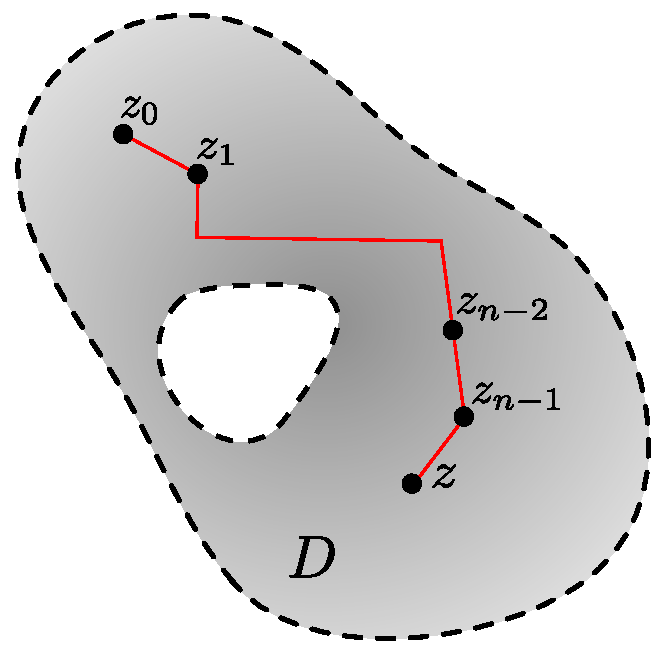
\includegraphics[scale = 0.5]{Figuras/DerivadaNula.pdf}
    \caption{Camino poligonal que une los puntos $z_0$ y $z$ de un abierto conexo $D$.}
    \label{fig:DerivadaNula}
\end{figure}

y, en consecuencia, $u(x_0,y_0) = u(x,y)$. Como $(x,y)$ es arbitrario, hemos probado que $u = cte$ para todo $z \in D$. De forma análoga, se prueba que $v$ es constante en $D$. Por lo tanto, $f$ es constante en $D$.
\end{proof}

\textbf{Observación:} La conexión de $D$ no puede ser omitida en la hipótesis del teorema. Por ejemplo, para el abierto no conexo $D = \{z \in \mathbb{C}: |z| < 2 \vee |z|> 3\}$, la función $f: D \rightarrow \mathbb{C}$ definida por
$$f(z) = \left\{ \begin{array}{cl}
     1,& \mbox{si} ~ |z|  < 2  \\
    0, & \mbox{si} ~ |z|  > 3
\end{array} \right. .$$

tiene derivada nula, pero no es constante.

\section{Funciones inversas*}

Al igual que el caso real, también se tiene un teorema de la función inversa. Antes de enunciar lo recordemos el teorema para variables reales en dos dimensiones:

\begin{teorema}\label{InversaCIII}
Si $f: A \subseteq \mathbb{R}^2 \longrightarrow \mathbb{R}^2$ es continuamente diferenciable en el abierto $A$ y $Jf(x_0,y_0)$ tiene determinante distinto de cero, entonces existen vecindades $U$ de $(x_0,y_0)$ y $V$ de $f(x_0,y_0)$ tales que $f: U \longrightarrow V$ es una biyección, $f^{-1}: V \longrightarrow U$ es diferenciable, y
$$Jf^{-1}(f(x,y)) = [Jf(x,y)]^{-1}.$$
\end{teorema}

\begin{teorema}[de la función inversa]
Sea $f: A \subseteq \mathbb{C} \longrightarrow \mathbb{C}$ analítica (con $f'$ continua) \footnote{Más adelante, por medio del teorema de Cauchy, veremos que  la analiticidad de la función implica directamente la continuidad de $f'$. } y suponga que $f'(z_0) \neq 0$. Entonces existe una vecindad $U$ de $z_0$ y una vecindad $V$ de $f(z_0)$ tal que $f: U \longrightarrow V$ es una biyección y su inversa $f^{-1}$ es analítica con su derivada dada por
$$\frac{d}{dw} f^{-1}(w) = \frac{1}{f'(z)}, \quad \forall w = f(z) \in V.$$
\end{teorema}

\begin{proof}
Por hipótesis, tenemos que $f(z) = (u(x,y), v(x,y)) = u(x,y) + iv(x,y)$ es analítica en $A$, entonces $u$ y $v$ satisfacen las ecuaciones de Cauchy-Riemann. Luego, la matriz Jacobiana está dada por
$$\forall (x,y) \in A: ~ Jf(x,y) = \begin{pmatrix}
\frac{\partial u}{\partial x} & \frac{\partial u}{\partial y} \\
\frac{\partial v}{\partial x} & \frac{\partial v}{\partial y}
\end{pmatrix}  = \begin{pmatrix}
\frac{\partial u}{\partial x} & -\frac{\partial v}{\partial x} \\
\frac{\partial v}{\partial x} & \frac{\partial u}{\partial x}
\end{pmatrix}$$

con determinante
$$\left(\frac{\partial u}{\partial x} \right)^2 + \left(\frac{\partial v}{\partial x} \right)^2 = |f'(z)|^2$$

ya que $f'(z) = u_x + i v_x $.  Ahora para $(x,y) = (x_0,y_0) = z_0$, se tiene que $f'(z_0) \neq 0$, por lo tanto, $|Jf(x_0,y_0)| = |f'(z_0)|^2 \neq 0$. Entonces, por el teorema de la función inversa para variable real, existen vecindades $U$ de $z_0$ y $V$ de $f(z_0)$ tales que $f: U \longrightarrow V$ es biyectiva. 

Basta probar que la inversa $f^{-1}: V \longrightarrow U$ es analítica. Para ello, consideremos la inversa de $Jf$:
$$\frac{1}{|Jf|} \begin{pmatrix} \frac{\partial v}{\partial y} & - \frac{\partial u}{\partial y} \\
-\frac{\partial v}{\partial x} & \frac{\partial u}{\partial x}
\end{pmatrix}.$$

Si escribimos $f^{-1}(x,y) = (t(x,y) , s(x,y)) =  t(x,y) + i s(t,y)$, entonces, comparando
$$J f^{-1} = \begin{pmatrix} \frac{\partial t}{\partial x} &  \frac{\partial t}{\partial y} \\
\frac{\partial s}{\partial x} & \frac{\partial s}{\partial y}
\end{pmatrix}$$

con la matriz inversa de $Jf$, obtenemos
\begin{align*}
    \frac{\partial t}{\partial x} &= \frac{1}{|Jf|} \frac{\partial v}{\partial y} = \frac{1}{|Jf|} \frac{\partial u}{\partial x}, \\
    \frac{\partial s}{\partial x} &= -\frac{1}{|Jf|} \frac{\partial v}{\partial x} = \frac{1}{|Jf|} \frac{\partial u}{\partial y}, \\
     \frac{\partial t}{\partial y} &= -\frac{1}{|Jf|} \frac{\partial u}{\partial y} = \frac{1}{|Jf|} \frac{\partial v}{\partial x}, \\
      \frac{\partial s}{\partial y} &= \frac{1}{|Jf|} \frac{\partial u}{\partial x} = \frac{1}{|Jf|} \frac{\partial v}{\partial y}.
\end{align*}

De esta forma hemos probado que para todo $(x,y) \in V$, se verifica que
\begin{align*}
    t_x &= s_y , \\
    t_y &= - s_x.
\end{align*}

Así las ecuaciones de Cauchy-Riemann se satisfacen para $t$ y $s$ ya que se satisfacen para las funciones continuamente diferenciables $u$ y $v$. Por lo tanto, $f^{-1}$ es analítica. Además, 
$$(f^{-1})'(w) = \frac{\partial t}{\partial x} + i \frac{\partial s}{\partial x} = \frac{1}{|Jf|} \left( \frac{\partial u}{\partial x} - i \frac{\partial v}{\partial x} \right) = \frac{\overline{f'(z_0)}}{|f'(z_0)|^2} = \frac{1}{f'(z_0)}, \quad w = f(z_0).$$
\end{proof}

\textbf{Observación:} El teorema de la función inversa nos garantiza la existencia de una inversa local para $f$. Por ejemplo, si consideramos $f(z) = z^2$ definida en $A = \mathbb{C} \setminus \{0\}$. Entonces $f'(z) = 2z \neq 0$ en cada punto de $A$. El teorema de la función inversa dice que $f$ tiene una inversa analítica local, que es simplemente alguna rama de la función raíz cuadrada. Pero $f$ no es inyectiva en todo $A$, pues, por ejemplo, $f(1) = f(-1)$.

\section{Funciones armónicas}

Recordemos que una función $h(x,y)$ a valores reales con dominio en el plano $xy$ se dice \textbf{armónica} si sobre ese dominio tiene derivadas parciales continuas de primer y segundo orden, y satisfacen la ecuación
$$\nabla^2 h = h_{xx}(x,y) + h_{yy} (x,y) = 0,$$

la cual es conocida como la \textbf{ecuación de Laplace}. Esta ecuación aparece en muchas ramas de la física tales como la astronomía, la electrostática, la mecánica de fluidos o la mecánica cuántica. Por ejemplo, si tenemos un sistema electrostático (cargas en reposo), el campo eléctrico puede ser escrito a partir de un potencial (electrostático) $\phi$ tal que $\Vec{E} = -\nabla \phi$. Reemplazando en la ley de Gauss en su forma diferencial:
$$\nabla \cdot \Vec{E} = \frac{\rho}{\varepsilon} \Rightarrow \nabla \cdot ( - \nabla \phi) = \frac{\rho}{\varepsilon}  \Rightarrow \nabla^2 \phi = -\frac{\rho}{\varepsilon},$$

es decir, el potencial satisface la \textbf{ecuación de Poisson}. Para regiones del espacio libre de fuentes de cargas, ésto es, $\rho \equiv 0$, el potencial satisface la ecuación de Laplace.
\\
 
Asumamos, ahora, que tenemos una función compleja y analítica
$$f(z) = u(x,y) + iv(x,y).$$

La pregunta que nos podemos hacer es si las funciones $u(x,y)$ y $v(x,y)$ son armónicas. La respuesta está en el siguiente teorema, el cual, para su demostración, se asumirá el siguiente resultado que será demostrado más adelante:

\begin{quote}
\textit{Las funciones componentes de una función analítica en un punto admiten derivadas parciales continuas de todos los órdenes en dicho punto.}
\end{quote}

\begin{teorema}
Si $f(z) = u(x,y) + iv(x,y)$ es analítica en un dominio $D$, entonces sus funciones componentes $u$ y $v$ son armónicas en $D$.
\end{teorema}

\begin{proof}
Dado que $f$ es analítica, las funciones componentes satisfacen las ecuaciones de Cauchy-Riemann en su dominio, ésto es,
\begin{eqnarray*}
u_x &=& v_y ,\\
u_y &=& -v_x .
\end{eqnarray*}

Derivando en ambos lados de las ecuaciones con respecto a $x$, tenemos:
\begin{eqnarray*}
u_{xx} &=& v_{yx}, \\
u_{yx} &=& -v_{xx}. 
\end{eqnarray*}

De igual manera, lo hacemos con respecto a $y$:
\begin{eqnarray*}
u_{xy} &=& v_{yy},\\
u_{yy} &=& -v_{xy} .
\end{eqnarray*}

Como las funciones componentes de $f$ tienen derivadas segundas continuas (porque $f$ es analítica), las derivadas cruzadas son iguales. Entonces,
\begin{eqnarray*}
u_{xx} &=& v_{yx} = v_{xy}, \\
u_{yy} &=& - v_{xy} = - v_{yx}, \\
v_{xx} &=& - u_{yx} = - u_{xy}, \\
v_{yy} &=& u_{xy} = u_{yx} .
\end{eqnarray*}

Por lo tanto,
$$u_{xx} + u_{yy} = 0 ~~\mbox{y}~~ v_{xx} + v_{yy} = 0,$$

es decir, $u$ y $v$ son armónicas.

\end{proof}

\begin{defi}
Si dos funciones $u(x,y)$ y $v(x,y)$ son armónicas en un dominio $D$ y sus derivadas parciales satisfacen las ecuaciones de Cauchy-Riemann en $D$; en otras palabras, la función $f = u + iv$ es analítica en $D$. Entonces  $v$ es llamada la \textbf{armónica conjugada} de $u$. 
\end{defi}

Es evidente que si una función $f(z) = u(x,y) + iv(x,y)$ es analítica en un dominio $D$, entonces $v$ es una armónica conjugada de $u$. Recíprocamente, si $v$ es una armónica conjugada de $u$ en un dominio $D$, la función $f$ es analítica en $D$. Ésto es consecuencia del teorema \ref{ECR} . Enunciamos este resultado como teorema.

\begin{teorema}
Una función $f(z) = u(x,y) + iv(x,y)$ es analítica en un dominio $D$ si y sólo si $v$ es una armónica conjugada de $u$.
\end{teorema}

\begin{ejemplo}
Consideremos las siguientes funciones definidas en el plano $xy$:
$$u(x,y) = x^2-y^2, \quad v(x,y) = 2xy.$$

Sus derivadas parciales son:
\begin{eqnarray*}
u_x = 2x; ~ v_y = 2x\\
u_y = -2y; ~ v_x = 2y
\end{eqnarray*}

Así, 
$$u_x = v_y ~~\mbox{y}~~ u_y = -v_x.$$

Pero,
$$v_x = - u_y ~~\mbox{y}~~ v_y = u_x,$$

es decir, no se cumplen las ecuaciones de Cauchy-Riemann. En consecuencia,
$$f(z) = x^2-y^2 + i2xy$$

es analítica en su dominio, entonces $v$ es la armónica conjugada de $u$, en cambio,
$$g(z) = 2xy + i(x^2-y^2)$$

no es analítica en punto alguno de su dominio, luego $u$ no es la armónica conjugada de $v$.
\end{ejemplo}

\begin{propo}

Algunas propiedades de las armónicas conjugadas son:

\begin{enumerate}
\item Si $v$ es armónica conjugada de $u$ y $u$ es armónica conjugada de $v$, entonces ambas funciones $u$ y $v$ son constantes.

\item Si $v$ es armónica conjugada de $u$, entonces $-u$ es armónica conjugada de $v$.

\item La función $f(z) = u(x,y) + iv(x,y)$  es analítica en su dominio si, y sólo si $if(z) = v(x,y) - iu(x,y)$ es analítica en dicho dominio.

\item Si $v$ y $w$ son armónicas conjugadas de $u$, entonces $v = w + C$, $C = cte$.
\end{enumerate}
\end{propo}

\begin{proof}
Queda como ejercicio para el lector.
\end{proof}

\textbf{Observación:} Es posible mostrar que toda función armónica definida en un cierto dominio tiene una armónica conjugada. Para determinarla, veamos el siguiente ejemplo.

\begin{ejemplo}
Sea  la función
$$u(x,y) = y^3-3x^2y.$$

Sus derivadas parciales segundas no cruzadas son:
$$u_{xx} = -6y, \quad u_{yy} = 6y. $$

Luego, $u$ es armónica para todo $(x,y) \in \mathbb{R}^2$. Notemos que si $v = v(x,y)$ es la armónica conjugada, entonces
$$u_x = -6xy = v_y.$$

Así,
$$v(x,y) = \int v_y dy = \int -6xy \,dy = -3xy^2 + C(x).$$

Ahora,
$$v_x = -3y^2 + C'(x) = -u_y = -3y^2 + 3x^2.$$

Entonces,
$$C'(x) = 3x^2 ~\Rightarrow~ C(x) = x^3 + c.$$

De esta manera,
$$v(x,y) = -3xy^2 + x^3 + c$$

es la armónica conjugada de $u$.
\end{ejemplo}

\textbf{Observación:} Por el ejemplo anterior, podemos construir funciones analíticas a partir de una función armónica. En ese caso,
$$f(z) = y^3 - 3x^2y + i(x^3 -3xy^2 + c) = i(z^3+c).$$

Por último, probemos el siguiente resultado:

\begin{quote}
    Dada una función armónica $u(x,y)$ definida sobre un dominio $D$ simplemente conexo\footnote{Un conjunto en el plano es \textit{simplemente conexo} si al tomar curvas cerradas dentro del conjunto, el interior sigue estando en el conjunto. En otras palabras, si el conjunto no posee agujeros.}, $u(x,y)$ admite siempre una armónica conjugada $v(x,y)$ en $D$.
\end{quote}

Recordemos del Cálculo III lo siguiente: Supongamos que $P(x,y)$ y $Q(x,y)$ tienen derivadas parciales de primer orden continuas en un dominio $D$ simplemente conexo del plano $xy$, y sean $(x_0,y_0)$ y $(x,y)$ dos puntos cualesquiera en $D$. Si $P_y = Q_x$ en todo punto de $D$, entonces el campo vectorial $\Vec{F} = (P,Q)$ es conservativo y la integral de línea
$$\int_C P(s,t) ds + Q(s,t) dt$$

desde $(x_0,y_0)$ hasta $(x,y)$, es independiente de la curva $C$ escogida, siempre que esté contenida en $D$. Además, si el punto $(x_0,y_0)$ se mantiene fijo y se permite que $(x,y)$ varíe sobre $D$, la integral representa una función univaluada
$$\phi(x,y) = \int_{(x_0,y_0)}^{(x,y)} P(s,t) ds + Q(s,t) dt$$

de $x$ e $y$ conocida como potencial de $\Vec{F}$, cuyas primeras derivadas parciales vienen dadas por las ecuaciones
\begin{equation}
  \frac{\partial \phi}{\partial x}(x,y) = P(x,y), ~ \frac{\partial \phi}{\partial y}(x,y) = Q(x,y).  \label{ArmoConj1}
\end{equation}

Notemos que el valor de $\phi$ cambia en una constante aditiva cuando se toma un punto $(x_0,y_0)$ diferente.

Volviendo a la función armónica dada $u(x,y)$, observemos que de la ecuación de Laplace $u_{xx} + u_{yy} = 0$ se sigue que
$$(-u_y)_y = (u_x)_x$$

en todo punto de $D$. Asimismo, como las segundas derivadas parciales de $u$ son continuas en $D$, las derivadas de primer orden de $-u_y$ y $u_x$ son continuas ahí. Así pues, si $(x_0,y_0)$ es un punto fijo de $D$, la función
$$v(x,y) = \int_{(x_0,y_0)}^{(x,y)} - u_t(s,t) ds + u_s(s,t) dt$$

está bien definida para todo $(x,y) \in D$, y de acuerdo con \eqref{ArmoConj1},
$$v_x(x,y) = - u_y(x,y),~ v_y(x,y) = u_x(x,y),$$

ésto es, $u$ y $v$ satisfacen las ecuaciones de Cauchy-Riemann. Como las derivadas de primer orden de $u$ son continuas, es evidente que las de $v$ también son continuas. Por tanto, $u+iv$ es una función analítica en $D$, y $v$ es, por consiguiente, una armónica conjugada de $u$. 

Claramente la función $v$ no es la única armónica conjugada de $u$. La función $v(x,y) + c$, con $c\in \mathbb{R}$ es también una armónica conjugada de $u$.